\chapter{Mathematical process model}
\label{chp:MathModel}

    The industrial scale production of highly pure oxygen and nitrogen as well as noble
    gases is still carried out by means of the cryogenic process.

    The initial process for production of pure oxygen first developed by Carl von Linde
    and first operated by Linde in 1902 \cite{Barron.1985} consisted of only
    a stripping section, in a way only half a rectification column. The reason for that is
    while it is easy to supply the heat necessary for the reboiler, a heat sink to operate
    a condenser at temperatures of about $95 K$ is not readily available on our planet.
    due to that highly pure oxygen could be withdrawn from the bottom of the column, but
    nitrogen was only produces at mediocre purities.

    The breakthrough that enabled operation of a ''full'' column, again developed by Linde in 1910,  was to operate the
    column sections at different pressures. That way the energy needed in the reboiler
    could be withdrawn from the condenser of the other column half. This leads to a
    somewhat inverted construction of the tower in comparison to regular distillation
    units, because the lower section forms the top section in this case and condenser
    and reboiler usually at the top and bottom of a column are combined in a single
    heat exchange unit in the middle of the column. This specialty of the process also
    leads to the need that the absolute values of the energies used in condenser and
    reboiler need to be equal. On terms of modelling the process this also forms a
    considerable challenge.

    \begin{figure}
        \begin{tikzpicture}
    \draw [arrow] (-4,0) -- (-2,0) node [pos=0.5,above] {} ;
    \draw [line width=1pt] (-2,0.75) rectangle (1,-0.75) node [align=center] at (-0.5,0) {\footnotesize pre- \\ \footnotesize purification} ;
    \draw [arrow] (1,0) -- (3,0) ;
    \draw [line width=1pt] (3,0.75) rectangle (6,-0.75) node [align=center] at (4.5,0) {\footnotesize compression \\ \footnotesize \& liquefaction};
    \draw [arrow] (6,0) -- (8,0) ;
    \draw [line width=1pt] (8,0.75) rectangle (11,-0.75) node at (9.5,0) {\footnotesize purification} ;
    \draw [arrow] (11,0) -- (13,0) ;
\end{tikzpicture}

        \caption{simplified cryogenic air separation process.}
        \label{fig:asu_simple}
    \end{figure}

    A simplified overview of the major process steps is given in \figref{fig:asu_simple}.
    Within the following sections the different process steps will be discussed in more detail.
    When appropriate the mathematical model for single process units is discussed as well.
    In addition to the separate process steps displayed in \figref{fig:asu_simple} the aspect
    of heat integration os essential to successfully operating an air separation unit (ASU).
    This aspect will be discussed separately as well (\secref{sec:heat_exchange})

    The pre-purification step of the process aim to reduce the amount of unwanted impurities
    from the ambient air as far as possible. The main sources of contamination are in this case
    dust and other organic components that can be found depending on the time of year and
    location of the plant. Furthermore are water and carbon dioxide common components in
    ambient air. The removal of these components is undertaken by means of adsorption molecular
    sieves such as zeolite or for initial steps coarser sieves. However the design and simulation
    of these pre-purification measures is not within the scope of this work. For more information
    the interested reader is referred to \cite{Acharya.1996}.


\section{Cryogenic air separation process }	
    The roots of cryogenic air separation lie in the first experiment and apparatus by Carl von Linde -- founder of the
    Linde AG -- which led to the first air separation plant in 1902. This earliest version of the an air separation plant
    consisted of a single column or one might argue even only half a column as it only possess a reboiler and no condenser).
    In 1910 the foundation of to the modern air separation was set with the development of a double column plant. There
    each column operated at different pressures, which enabled the condenser and reboiler to be combined into a
    single heat exchange unit. This basic principle is in use to this day. However several enhancements have been made to
    to the original process design. Some were driven by new technological developments. Among the most prominent is the
    recovery of pure Argon -- only a trace element in ambient air -- within the process. Initially the Argon recovery
    had to be undertaken through the help of a catalytic converter. With the development of structured packings which
    display a very low pressure drop and height equivalent to theoretical stage (HEPT) it became feasible to separate
    Argon within a separate distillation column, as it requires a lot of theoretical stages, which would have
    previously led to infeasible large towers. Further advancements include internal compression which allows
    for compression of liquefied products within the cold box and more advanced designs of the condenser / reboiler unit.

    \begin{figure}
        \centering
        \begin{tikzpicture}[scale=0.9]
    \draw [arrow] (-1,1) node (start) [inner sep=0] {} -- ++(2.5,0) node [pos=0.5,above,yshift=-1mm] {plant air} -- ++(0,-1) node (CompIn) [inner sep=0] {};
    
    % box 3 stage compression
    \pgfmathsetmacro{\halfboxwidth}{1.5}
    \pgfmathsetmacro{\boxheight}{1.5}
    \draw [stdline] (CompIn) -- ++(\halfboxwidth,0) -- ++(0,-\boxheight) -- ++(-\halfboxwidth,0) node (CompOut) [pos=1,inner sep=0] {} -- ++(-\halfboxwidth,0) -- ++(0,\boxheight) -- cycle ;
    \node [align=center] at ($ (CompIn) - 0.5*(0,\boxheight)$) {3 stage \\ compression} ;
    
    % connection compression splitter
    \draw [arrow] (CompOut) -- ++(0,-0.5) node (SplitIn) [pos=1,inner sep=0] {};
    
    % splitter
    \draw [stdline] (SplitIn) -- ++(0.35,-0.6) -- ++(-0.7,0) node (SplitOut1) [inner sep=0cm,pos=0.2] {} node (SplitOut2) [inner sep=0cm,pos=0.8] {} -- cycle ;
    
    % multi stream heat exchanger 
    \pgfmathsetmacro{\hxheight}{2.5}
    \pgfmathsetmacro{\hxwidth}{3}
    \draw [stdline] (0,-5) node (HXstart) {} -- ++(\hxwidth,0) node (HX1) [inner sep=0cm,pos=0.166] {} node (HX2) [inner sep=0cm,pos=0.333] {} node (HX3) [inner sep=0cm,pos=0.5] {} node (HX4) [inner sep=0cm,pos=0.666] {} node (HX5) [inner sep=0cm,pos=0.8333] {} -- ++(0,-\hxheight) node (HXS) [pos=0.5,inner sep =0cm] {}-- ++(-\hxwidth,0) node (HX6) [inner sep=0cm,pos=0.333] {} node (HX7) [inner sep=0cm,pos=0.5] {} node (HX8) [inner sep=0cm,pos=0.666] {} node (HX9) [inner sep=0cm,pos=0.8333] {} -- cycle ;
    \draw [grdash] (HX5) -- (HX5 |- HXS) -- (HXS) ;
    \draw [grdash] (HX4) -- (HX6) ;
    \draw [grdash] (HX7) -- (HX3) ;
    \draw [grdash] (HX8) -- (HX2) ;
    \draw [grdash] (HX9) -- (HX1) ;
    \node [align=center] at ($(HXstart) + 0.5*(\hxwidth,-\hxheight)$) {multi - stream \\ heat exchanger} ;
    
    %connection splitter heat exchanger
    \draw [arrow] (SplitOut1) -- ++(0,-0.25) node (a) {} -- (a -| HX5) -- (HX5) ;
    \draw [arrow] (SplitOut2) -- ++(0,-0.5) node (b) {} -- (b -| HX4) -- (HX4) ;
    
    % tower LPC column
    \pgfmathsetmacro{\towerheight}{5}
    \pgfmathsetmacro{\towerwidth}{2}
    \pgfmathsetmacro{\domerad}{0.84*\towerwidth/2}
    \draw [line width=1pt, rounded corners] (7,-4.5) node (LPCstart) {} -- ++(0,\towerheight) .. controls +(76:\domerad) and +(104:\domerad) .. ++(\towerwidth,0) node (LPCtopIn) [inner sep=0cm , pos=1.0] {} node (A) [inner sep=0cm , pos=0.5] {} -- ++(0,-\towerheight) .. controls +(-104:\domerad) and +(-76:\domerad) .. ++(-\towerwidth,0) node (B) [inner sep=0cm , pos=0.5] {} -- cycle ;
    \node at ($(LPCstart) + 0.5*(\towerwidth,\towerheight)$) {LPC} ;
    
    % tower HPC column
    \pgfmathsetmacro{\towerheight}{3}
    \pgfmathsetmacro{\towerwidth}{2}
    \pgfmathsetmacro{\domerad}{0.84*\towerwidth/2}
    \draw [line width=1pt, rounded corners] (7,-9) node [inner sep=0] (HPCstart) {}-- ++(0,\towerheight) .. controls +(76:\domerad) and +(104:\domerad) .. ++(\towerwidth,0) node (HPCtopOut2) [inner sep=0cm , pos=0.0] {} node (HPCtopOut) [inner sep=0cm , pos=1.0] {} -- ++(0,-\towerheight) .. controls +(-104:\domerad) and +(-76:\domerad) .. ++(-\towerwidth,0) node (D) [inner sep=0cm , pos=0.5] {} -- cycle ;
    \node at ($(HPCstart) + 0.5*(\towerwidth,\towerheight)$) {HPC} ;

    % evaporator 
    \draw [fill = white,line width = 1pt] (8.75,-4.5) rectangle (7.25,-6.00) ;
    \draw [line width = 0.75pt] (7.25,-6.00) -- ++(0.4,1.3) -- ++(0.7,0) -- ++(0.4,-1.3) ;
    \draw [line width = 0.75pt] (7.25,-4.9) -- ++(1.3,0) -- ++(0,-0.25) -- ++(-1.1,0) -- ++(0,-0.20) -- ++(1.1,0) -- ++(0,-0.25) -- ++(-1.3,0) ;
    
    % connection HX -- expander 
    \draw [arrow] (HXS) -- ++(0.5,0) node [inner sep = 0cm] (c) {};
    
    % expander 
    \draw [stdline] (c) -- ++(0,0.75) -- ++(0.75,0.25) node (Eaus) [pos=1,inner sep =0cm] {} -- ++(0,-1.25) -- cycle ;
    
    % connection expander valve 1
    \draw [arrow] (Eaus) -- ++(0,2) node (V1in) [inner sep =0cm] {} ;
    
    % valve 1
    \draw [stdline] (V1in) -- ++(-0.25,0) -- ++(0.5,0.75) -- ++(-0.5,0) node (V1out) [inner sep=0cm,pos=0.5] {} -- ++(0.5,-0.75) -- cycle ;
    
    % connection valve 1 -- LPC 
    \draw [arrow] (V1out) -- ++(0,1.5) node (d) [inner sep=0cm] {} -- (d -| LPCstart) node (LPCin) [pos=0.3] {};
    
    % connection HX -- HPC
    \draw [arrow] (HX6) -- (HX6 |- HPCstart) node (f) [pos=0.75] {} node (g) [pos=0.5] {} -- (HPCstart) ;
    
    % connection LPC top -- HX : gaseous nitrogen 
    \draw [stdline] (A) -- ++(0,0.5) node (e) {} -- (LPCin |- e) -- (LPCin) ;
    \draw [stdline] (LPCin) -- (LPCin |- f) -- (f) ;
    \draw [arrow] (f) -- (HX8 |- f) -- (HX8) ;
    
    \draw [arrow] (HX3) -- ++(0,1.5) node (O2Out) {} -- (O2Out -| start) node [pos=0.5,above,yshift=-1mm] {\footnotesize $G-O_2$};
    \draw [arrow] (HX2) -- ++(0,1.0) node (N2Out) {} -- (N2Out -| start) node [pos=0.5,above,yshift=-1mm] {\footnotesize $G-N_2$};
    \draw [arrow] (HX1) -- ++(0,0.5) node (waste) {} -- (waste -| start) node [pos=0.5,above,yshift=-1mm] {\footnotesize waste};
    
    % connection HPC -- LPC 
    \draw [arrow] (HPCtopOut) -- ++(2,0) -- ++(0,5) node (V2in){} ;
    \draw [stdline] (V2in) -- ++(-0.25,0) -- ++(0.5,0.75) -- ++(-0.5,0) node (V2out) [inner sep=0cm,pos=0.5] {} -- ++(0.5,-0.75) -- cycle ;
    \draw [arrow] (V2out) -- (V2out |- LPCtopIn) -- (LPCtopIn) ;
    
    % connection HPC top -- HX 
    \node (i) at (LPCin |- g) {} ;
    \draw [stdline] (HPCtopOut2) -- ++(-1.0,0) node (h) {} -- (g -| h) -- (i) ;
    \draw [stdline] (i) -- (g) ;
    \draw [arrow] (g) -- (g -| HX7) -- (HX7) ;
    
    % connection HPC waste 
    \node (LPCwaste) [inner sep=0] at ($(LPCin -| LPCtopIn) + (0,0.75)$) {} ;
    \node (j) at ($(HPCtopOut) + (1,0)$) {} ;
    \node (k) [inner sep=0] at ($(D -| j) - (0,1)$) {} ;
    \draw [stdline] (LPCwaste) -- ++(1,0) -- (j) ;
    \draw [arrow] (j) -- (k) -- (HX9 |- k) -- (HX9) ;
    
    % tower ArC
    \pgfmathsetmacro{\towerheight}{5}
    \pgfmathsetmacro{\towerwidth}{1.5}
    \pgfmathsetmacro{\domerad}{0.84*\towerwidth/2}
    \draw [line width=1pt, rounded corners] (12.5,-4) node [inner sep=0] (ArCstart) {}-- ++(0,\towerheight) .. controls +(76:\domerad) and +(104:\domerad) .. ++(\towerwidth,0) node (ArCtopOut) [inner sep=0cm , pos=0.5] {} node (ArCtopOut2) [inner sep=0cm , pos=1] {} -- ++(0,-\towerheight) .. controls +(-104:\domerad) and +(-76:\domerad) .. ++(-\towerwidth,0) node (ArCbot) [inner sep=0cm , pos=0.5] {} -- cycle ;
    \node at ($(ArCstart) + 0.5*(\towerwidth,\towerheight)$) {ArC} ;
    
    % connection LPC -- ArC
    \node (ArCout) [inner sep=0] at (ArCstart -| LPCtopIn) {} ;
    \node (ArIn) [inner sep=0] at ($(ArCout) - (0,0.25)$) {};
    \node (l) at (ArCstart -| k) {} ;
    \node (m) at (ArCstart -| V2in) {} ;
    \node (n) [inner sep=0] at ($(m) + (1,-0.25)$) {} ;
    \node (o) [inner sep=0] at ($(ArCbot) - (0,0.5)$) {} ;
    \node (p) at ($(m) - (0,0.25)$) {} ;
    \node (q) at ($(l) - (0,0.25)$) {} ;
    \draw [stdline] (ArCout) -- (l) ;
    \draw [stdline] (l) -- (m) ;
    \draw [arrow] (m) -- (ArCstart) ; 
    \draw [stdline] (ArCbot) -- (o) -- (o -| n) -- (n) -- (p) ;
    \draw [stdline] (p) -- (q) ;
    \draw [arrow] (q) -- (ArIn) ;
    
    % ArC heater 
    \node (ArCheat) [black,draw,circle,fill=white,minimum size=1.2cm] at ($(ArCtopOut) + (1.5,0.5)$) {} ; 
    \draw [stdline] (ArCtopOut) --  (ArCheat -| ArCtopOut) -- (ArCheat.west) ;
    \draw [arrow] (ArCheat.south) -- (ArCheat |- ArCtopOut2) -- (ArCtopOut2) ; 
    
    %connection HPC ArC heater 
    \node (r) [inner sep=0] at ($(D) - (0,0.5)$) {} ;
    \node (s) at (r -| k) {} ;
    \draw [stdline] (D) -- (r) -- (s) ;
    \node (t) [inner sep=0] at ($(ArCheat.east) + (0.75,1)$) {} ;
    \node (u) at ($(LPCin) + (1,0)$) {} ;
    \node (v) at (e -| u) {} ;
    \draw [arrow] (s) -- (t |- s) -- ++(0,4) node (V3in) {} ;
    \draw [stdline] (V3in) -- ++(-0.25,0) -- ++(0.5,0.75) -- ++(-0.5,0) node (V3out) [inner sep=0cm,pos=0.5] {} -- ++(0.5,-0.75) -- cycle ;
    \draw [stdline] (V3out) -- (t) -- ++(-1.1,0) -- ++(0,-1.2) -- ++(-0.2,0.2) -- ++(-0.2,-0.2) -- ++(0,1.2) -- (u |- t) -- (v) ;
    \draw [stdline] (v) -- (u) ;
    \draw [arrow] (u) -- ++(0,-1.5) node (w) {} -- (LPCstart |- w) ;
    \node (x) at (t |- ArCtopOut2) {} ;
    \draw [stdline] (ArCheat |- ArCtopOut2) -- (x) ;
    \draw [arrow] (x) -- ++(1,0) ;
\end{tikzpicture}



        \caption{simplified cryogenic air separation process.}
        \label{fig:ASU_simple_coco}
    \end{figure}

    For the purposes of this project a simplified version of an ASU has been considered. A process flowsheet is depicted
    in \figref{fig:ASU_simple_coco}.

    \subsection{Flowsheet initialization}
        Even for single unit models initialization might pose difficulties, when a whole process model is considered,
        this task might become even more difficult. If the process units are mainly sequential, the task of initializing
        becomes no more difficult, then initializing the single units. But in most chemical processes a purely sequential
        arrangement of process equipment is not given. As soon as feedbacks are introduced into the process, the question
        of initialization becomes considerably more complex. In the most general case it is not even ensured, that a steady
        state of process operations even exists. As feedbacks are introduced, the process might become unstable or display
        oscillatory behaviour. \Figref{fig:foreward_process} shows the concept for a purely feed forward process, while
        \figref{fig:feedback_process} is an example for a process with feedbacks, in particular an arrangement with an inner
        and outer feedback loop.

        \begin{figure}
            \centering
            \begin{subfigure}{0.4\textwidth}
                \begin{tikzpicture}
    \draw [arrow] (0,0) -- (1.5,0) ;
    \draw [stdline] (1.5,0.5) rectangle (3,-0.5) node at (2.25,0) {unit 1} ;
    \draw [arrow] (3,0) -- (4.5,0) ;
    \draw [stdline] (4.5,0.5) rectangle (6,-0.5) node at (5.25,0) {unit 2} ;
    \draw [arrow] (6,0) -- (7.5,0) ;
    \draw [white] (0,0.5) -- (0,-1.7) ;
\end{tikzpicture}

                \caption{Feed forward process.}
                \label{fig:foreward_process}
            \end{subfigure}
            \hspace{0.05\textwidth}
            \begin{subfigure}{0.4\textwidth}
                \begin{tikzpicture}
    \draw [arrow] (0,0) -- (0.6,0) ;
    \draw [arrow] (0.9,0) -- (1.5,0) ;
    \draw [stdline] (0.75,0.15) -- ++(0.15,-0.15) -- ++(-0.15,-0.15) -- ++(-0.15,0.15) -- cycle ;
    \draw [stdline] (0.75,-1) -- ++(0.15,-0.15) -- ++(-0.15,-0.15) -- ++(-0.15,0.15) -- cycle ;
    \draw [stdline] (1.5,0.5) rectangle (3,-0.5) node at (2.25,0) {unit 1} ;
    \draw [arrow] (3,0) -- (3.6,0) ;
    \draw [arrow] (3.9,0) -- (4.5,0) ;
    \draw [stdline] (3.75,0.15) -- ++(0.15,-0.15) -- ++(-0.15,-0.15) -- ++(-0.15,0.15) -- cycle ;
    \draw [arrow] (3.75,-0.15) -- (3.75,-1.15) -- (0.9,-1.15) ;
    \draw [stdline] (4.5,0.5) rectangle (6,-0.5) node at (5.25,0) {unit 2} ;
    \draw [arrow] (6,0) -- (6.6,0) ;
    \draw [arrow] (6.9,0) -- (7.5,0) ;
    \draw [stdline] (6.75,0.15) -- ++(0.15,-0.15) -- ++(-0.15,-0.15) -- ++(-0.15,0.15) -- cycle ;
    \draw [arrow] (6.75,-0.15) -- (6.75,-1.7) -- (0.75,-1.7) -- (0.75,-1.3) ;
    \draw [arrow] (0.75,-1) -- (0.75,-0.15) ;
    \draw [white] (0,0.5) -- (0,-1.7) ;
\end{tikzpicture}

                \caption{process with feedbacks.}
                \label{fig:feedback_process}
            \end{subfigure}
            \caption{Different process configurations.}
        \end{figure}

        As mentioned before feedbacks greatly complicate calculations for a given process. With the cryogenic air separation
        process this is especially true, since it is highly integrated and coupled. The only external cooling that is available
        comes from the initial compression and expansion of the ambient air. During the compression, since temperatures are
        still around ambient conditions and conventional coolants can be employed as heat sink. This is done during the
        multi-stage compression. All other heat exchange within the process can only be done against other internal process
        streams, as the process operates at conditions far away form ambient conditions. Far more than the feedbacks associated
        with material streams, it is the energy coupling that makes simulation of this process a non-trivial task. Especially, as
        the energies in condenser and reboiler of distillation columns have great effects on all operating condition.

        \begin{figure}
            \centering
            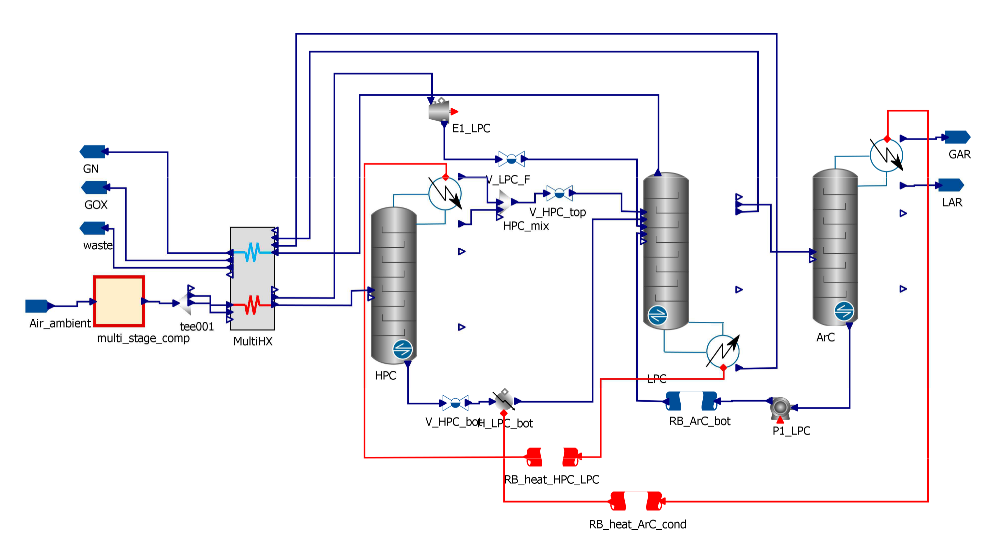
\includegraphics[width=0.9\textwidth]{Pictures/ASU_simple_gPROMS.eps}
            \caption{Implementation of simplified cryogenic air separation process in gPROMS.}
            \label{fig:ASU_simple_gproms}
        \end{figure}

        \Figref{fig:ASU_simple_gproms} shows the flowsheet of the simplified ASU process depicted in \figref{fig:ASU_simple_coco}.
        In order the symbols in the material streams (blue) and energy streams (red) represend so called recycle breakers, which
        play a vital role during initialization of the flowsheet. The recycle breakers play no part in the converged flowsheet.
        Their function is to break the recycle or feedback loops in the process and transform the process into a feed forward process
        during initial computations. To achieve that, the recycle breakers are supplied with initial guesses for for all properties
        associated with the respective material or energy streams. For the energy recycle breakers the transformation from open to
        closed operation mode is rather simple. The outlet energy stream is merely moved from initial guess to inlet stream by
        means of \eqref{eq:homotopy}. For the material breaker one hast to invest a little more effort, as not all properties can be
        moved so easily while maintaining physical sense. The material stream and pressure are treated identically, while the temperature
        needs to computed from an enthalpy balance.

        As for the concrete initialization procedure: first all recycle breakers are open and have the initial guesses at their outlet
        ports. Then all single units are converged. While this is done simultaneously in terms of the solution algorithm, the downstream
        units remain in the simplified stages of the unit respective initialization procedures wile the upstream units are solved with the
        rigorous models. Once all units have been converged, the recycle breakers are closed one after another. First the material stream
        between the Argon column (ArC) and the low pressure column (LPC), then the energy couple between the Argon condenser and
        and the oxygen rich material stream is closed. Finally the -- maybe most important -- connection between the LPC reboiler
        and HPC condenser is established.
